\documentclass[main]{subfiles}


\begin{document}
	\begin{lect} {2019-09-30}

\subsection{Вычисление кручения}

		\begin{Reminder}
			\[(\vec{a}; \vec{b}; \vec{c}) = (\vec{a}; \vec{b}; \vec{c} + \alpha \vec{a})\]
			\[k = \frac{\abs{f' \times f''}}{\abs{f'}^3}\]
		\end{Reminder}

	  \begin{Theorem}
	    \[g(s) \text{ - нат. парам., тогда:}\]
	    \[\ae = \frac{(g', g'', g''')}{k ^ 2}\]
	  \end{Theorem}
		\begin{Proof}

			\[g'(s) = \vec{v} \q\q \abs{\vec{v}} = 1\]
			\[g''(s) = v' = k \vec{n}\]
			\[g'''(s) = kn' = k(-k \vec{v} + \ae \vec{b}) = -k^2 \vec{v} + \ae k \vec{b}\]
			\[(g', g'', g''') = (\vec{v}; k \vec{n}; -k^2 \vec{v} + \ae k \vec{b}) =
			(v; kn; \ae k b) = \ae k^2\]
			\[\Ra \ae = \frac{(g', g'', g''')}{k ^ 2}\]
		\end{Proof}

	  \begin{Theorem}
	    \[f(t) \text{ - парам $(\forall)$, тогда: }\]
	    \[\ae = \frac{(f', f'', f''')}{\abs{f' \times f''}^2}\]
	  \end{Theorem}

		\begin{Proof}
		    \[f(t) \text{ - парам } (\forall)\]
			\[s = \psi(t) = \int_a^t \abs{f'(\tau)} d\tau \q\q g(s) \text{ - нат. парам}\]
			\[\psi'(t) = \abs{f'(t)}\]
			\[g(s) = g(\psi(t)) = f(t)\]
			\[f'(t) = g'(\psi(t)) \cdot \psi'(t) = g'(s) \cdot \abs{f'(t)}\]
			\[f''(t) = g''(\psi(t))(\psi'(t))^2 + g'(\psi(t))\psi''(t) = g''(s) \cdot \abs{f'(t)}^2 +
			g'(s) \cdot \psi''(t)\]
			\[f'''(t) = g'''(\psi(t))(\psi'(t))^3 + g''(\psi(t)) \cdot 3 \psi'(t) \psi''(t) +
			g'(\psi(t)) \cdot \psi'''(t)\]
			\[(f', f'', f''') = (\vec{g'}(s) \cdot \abs{f'(t)}; \  \vec{g}''(s) \abs{f'(t)}^2,
			g'''(s) \cdot \abs{f'(t)} ^3) = \]
			\[ = (g', g'', g''') \cdot \abs{f'(t)}^6\]
			\[\ae = \frac{(g', g'', g''')}{k^2} = \frac{(f', f'', f''')}{\abs{f'(t)}^6} \cdot
			\frac{\abs{f'(t)} ^6}{\abs{f' \times f''}^2} = \frac{(f', f'', f''')}{\abs{f' \times f''}^2}\]
		\end{Proof}

		\begin{Example}
			\[\begin{cases}
					x = t\\
					y = f(t)
			\end{cases}\]
			\[y = f(x) \q\q \vec{f} = (x; f(x); 0) \q\q \vec{f}'(1; f'(x); 0) \q\q f''(0; f''(x); 0)\]
			\[f'''= (0; f'''(x); 0)\]
			\[k = \frac{\abs{f''(x)}}{(1 + f'^2(x))^{\frac{3}{2}} }\]
			\[f' \times f'' = (0; 0; f''(x))\]
			\[\ae = 0\]
		\end{Example}

\subsection{Теорема о соприкасающейся плоскостии}

		\begin{definition}
			\begin{figure}[H]
			    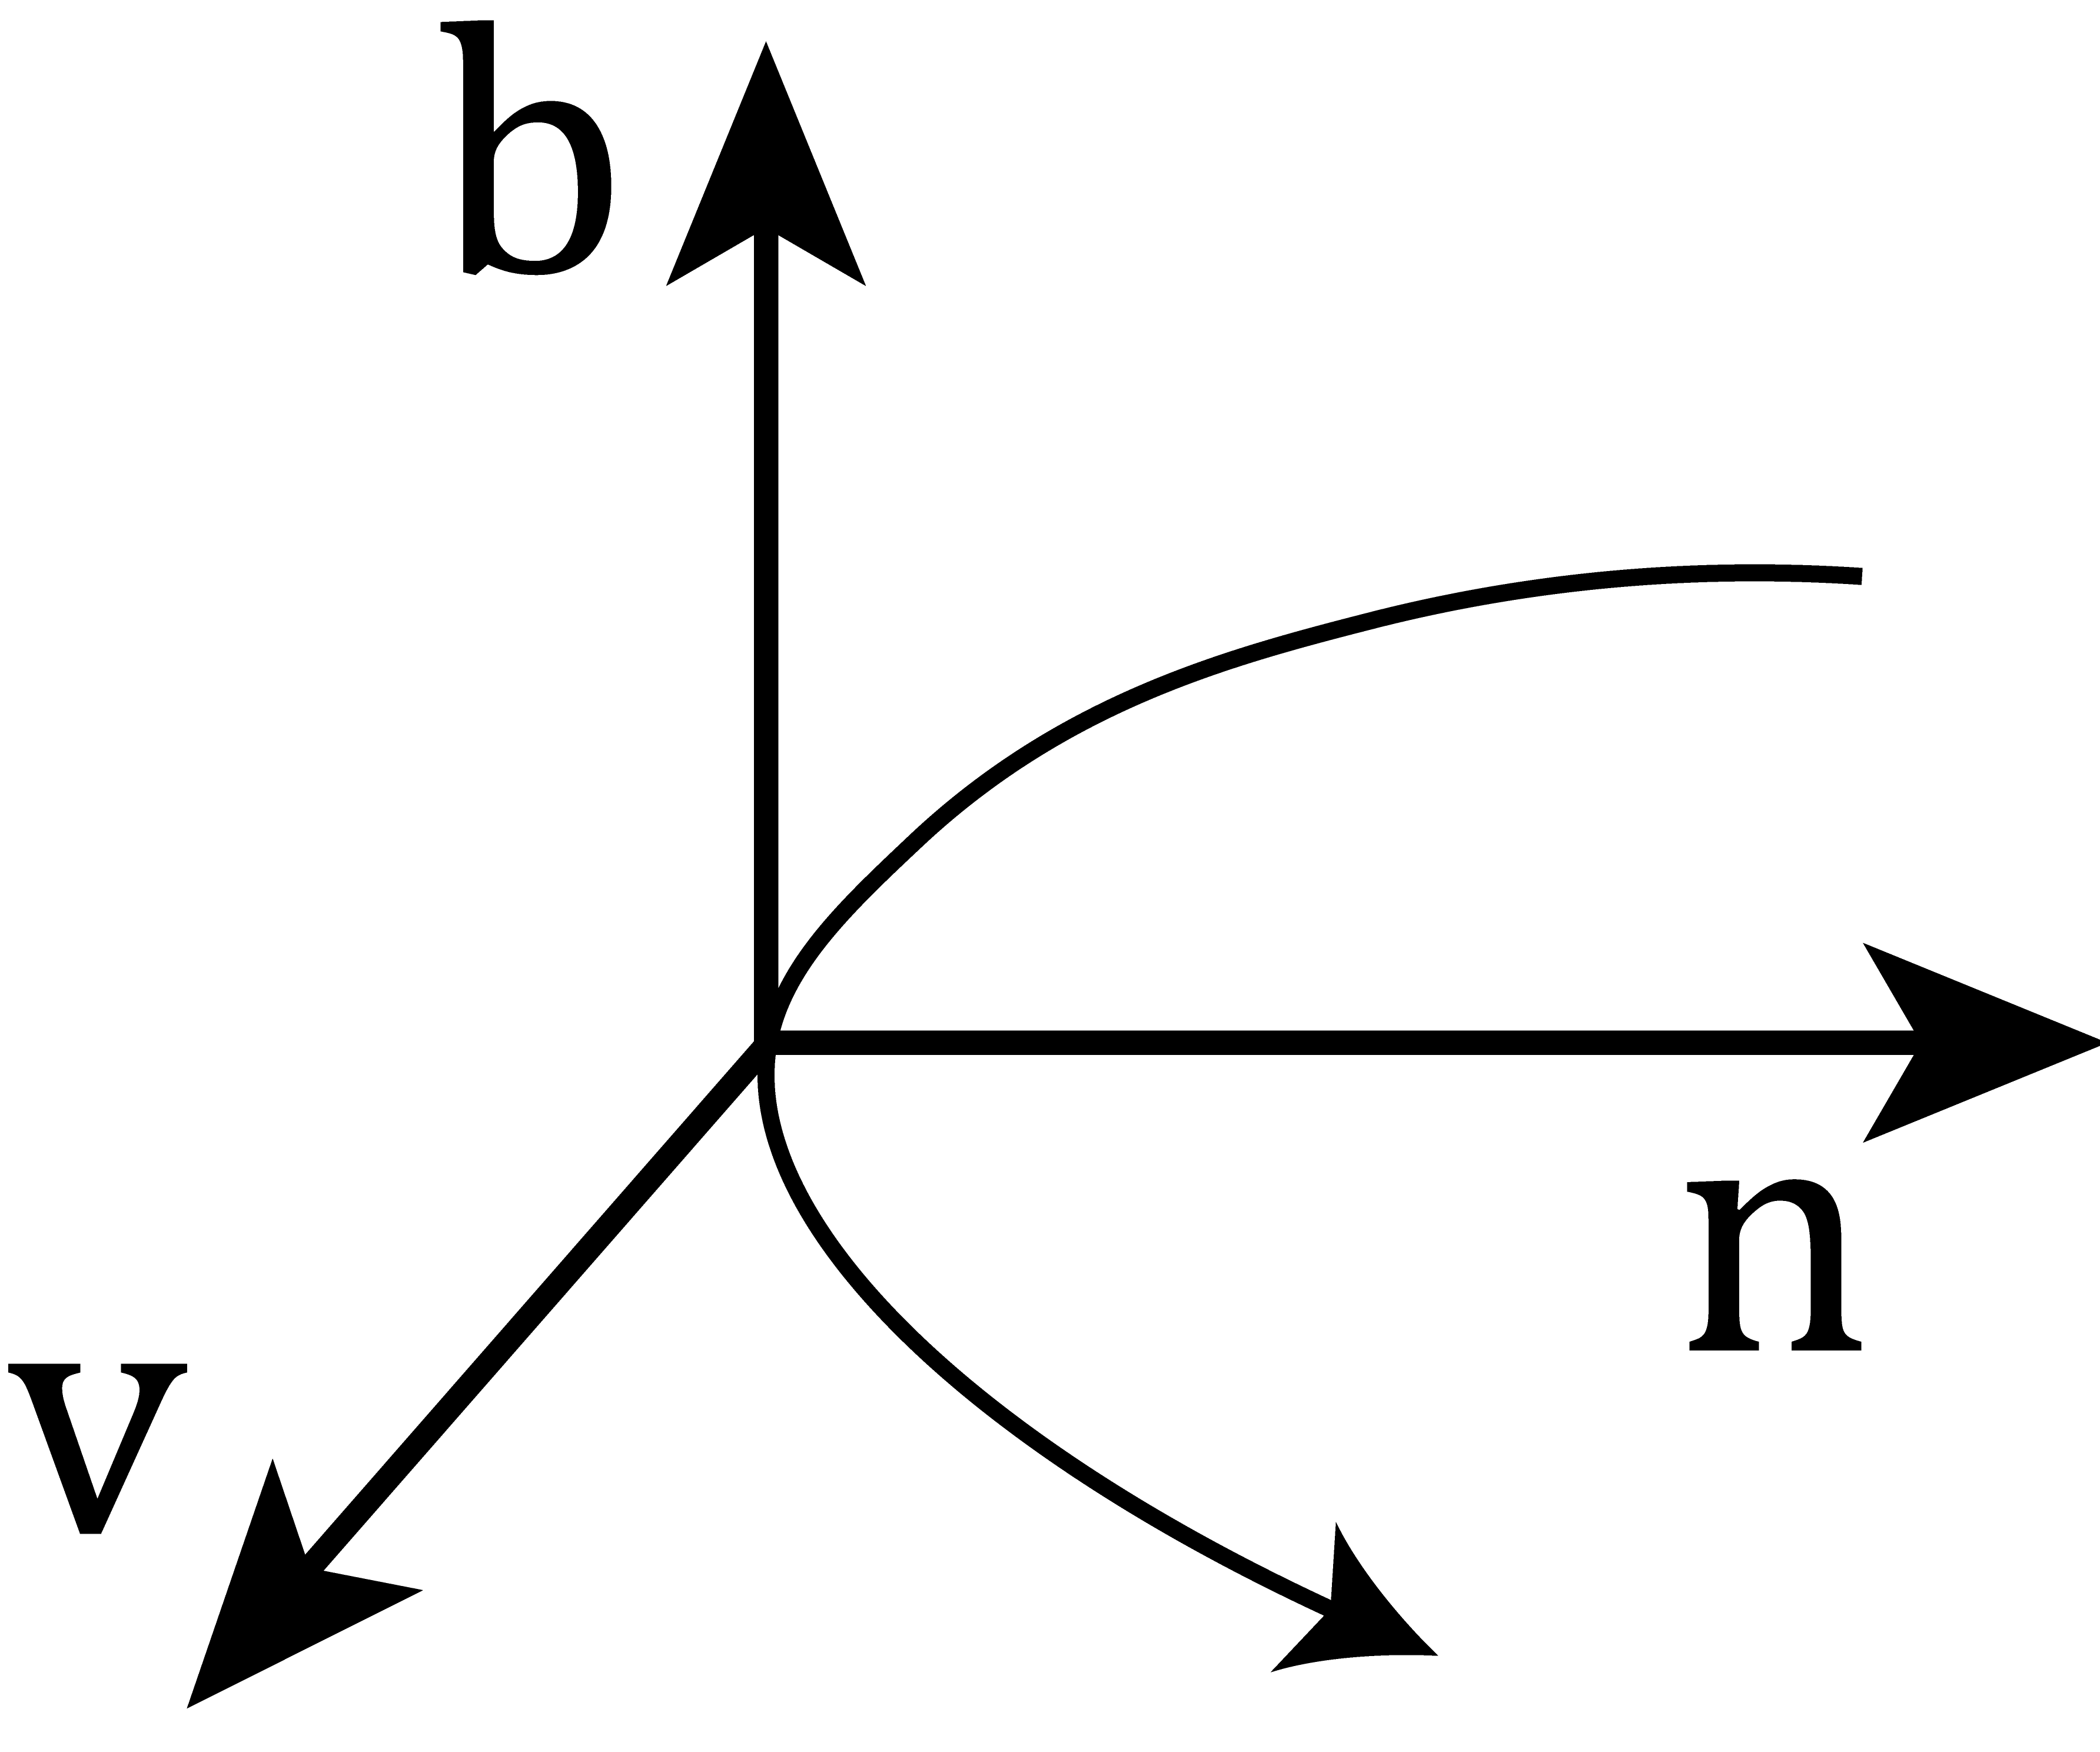
\includegraphics[width=4cm]{pics/4_1.png}
			    \centering
			\end{figure}

		    Соприкас плоскость : $<\vec{v}, \vec{n}>$\\
			Нормальная плоскость кривой : $<n, b>$\\
			Спрямляющая плоскость : $<v, b>$
		\end{definition}

		\begin{Theorem}
			\[\vec{f}(t) = (f_1(t); f_2(t); f_3(t))\]
			Уравнение нормальной плоскости:
			\[\vec{v} \parallel f'(t) = (f_1', f_2', f_3')\]
            \[f'_1(t_0) \cdot(x - f_1(t_0)) +
			f_2'(t_0) \cdot (y - f_2(t_0)) + f'_3(t_0) \cdot (z - f_3(t_0)) = 0\]
			\[f' \times f'' \parallel b\]
			так как ЛНЗ
			\[(f'_1, f'_2, f'_3) \times (f''_1, f''_2, f''_3) = (f'_2 f''_3 - f'_3 f''_2;
			f'_3 f_1'' - f'_1 f''_3; f'_1 f''_2 - f'_2 f''_1)\]
			Соприкас плоск.
			\[\begin{vmatrix}
				f'_1(t_0) & f_2'(t_0) & f'_3(t_0)\\
				f_1''(t_0) & f''_2(t_0) & f''_3(t_0)\\
				x - f_1(t_0) & y - f_2(t_0) & z - f_3(t_0)
			\end{vmatrix} = 0\]
			\[(f'(t_0) \times f''(t_0)) \times f'(t_0) \parallel \vec{n}\]
			Ур-е спрям. плоск - УПР
		\end{Theorem}

		\begin{Theorem}
			\begin{figure}[H]
			    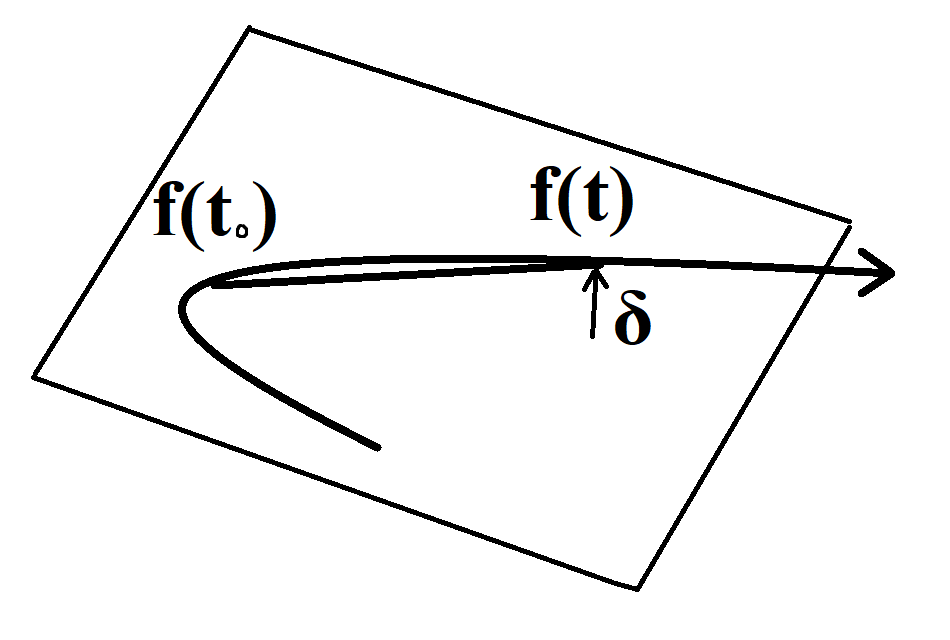
\includegraphics[width=6cm]{pics/4_2.png}
			    \centering
			\end{figure}

			\[\delta \text{ - расст. от } f(t) \text{ до соприкас. плоскости}\]
			Если плоскость явл. соприкас., то
			\[\lim_{t \to t_0} \frac{\delta}{\abs{f(t) - f(t_0)}^2} = 0 \]
			Плоскость с таким соотношением ед.
		\end{Theorem}

		\begin{proof}
			 Условия достигаются за счет подходящей системы координат
			\[a) \q f(t_0) = (0, 0, 0)\]
			\[b) \q OX \parallel \vec{v}(t_0)\]
			\[c) \q OY \parallel \vec{n}(t_0)\]
			\[d) \q t_0 = 0\]
			\[e) \q t \text{ - нат. параметр} \]
			\[\text{б, в } \Ra OZ \parallel \vec{b}(t_0)\]

			\[f(t) = (f_1(t); f_2(t) ; f_3(t)) \Ra \delta = \abs{f_3(t)}\]
			Соприкас $z = 0$
			\[\vec{v} \parallel f' = (f'_1, f'_2, f'_3) \parallel OX \Ra f'_2(0) = 0, \q f'_3(0) = 0 \q
			f'_1(0) \neq 0\]
			\[\vec{n} \parallel f'' = (f''_1, f_2'', f_3'') \parallel OY \Ra f''_1(0) = 0; \q f''_3(0) = 0\]
			 Следует из пункта e)
			\[\text{Хотим } \lim_{t \to 0} \frac{\abs{f_3(t)}}{\abs{f(t)}^2} = 0\]
			\[\lim_{t \to 0} \frac{f_3(t)}{f_1(t)^2 + f_2(t)^2 + f_3(t)^2} \os{\text{Лопиталь}}{=}
            \]
            \[= \lim_{t \to 0} \frac{f'_3(t)}{2 f_1(t) f_1'(t) + 2f_2(t)f'_2(t) + 2f_3(t) f'_3(t)} \os{\text{Лопиталь}}{=}\]
			\[= \frac{1}{2} \lim_{t \to 0} \frac{f''_3(t)}{
			f'_1^2(t) + f_1(t) f''_1(t) +
			f_2'(t)^2 + f_2(t)f_2''(t) +
			f'_3^2(t) + f_3(t)f''_3(t)} \]
			Все кроме первого слагаемого в знаменателе стремятся к 0, числитель тоже стремится к 0. Замечание. Можно было разложить $f_1,f_2,f_3$ по Тейлору. Можно зачеркнуть пункт д(e)) и $f_1''(0)=0$
		\end{proof}

		\subsection{Натуральные уравнения кривой.}
		\begin{Theorem}
			\[g_1(s) \text{  и } g_2(s) \text{ - нат. парам. двух кривых}\]
			\[\begin{align}
				&k_1(s) & k_2(s)\\
				&\ae_1(s) & \ae_2(s)
			\end{align} \text{ - кривизны и кручения}\]
			\[\begin{align}
				\text{Если }& k_1(s)   = k_2(s)\\
							& \ae_1(s) = \ae_2(s)
			\end{align} \Ra \text{ кривые наклад. при движении пр-ва}\]
		\end{Theorem}

		\begin{Proof}
			\[v_1(s), n_1(s), b_1(s) \text{ - базис Френе \RNumb{1} кривой}\]
			\[v_2(s), n_2(s), b_2(s) \text{ - базис Френе \RNumb{2} кривой}\]
			\[\begin{align}
                \text{Считаем }& v_1(s_0) = v_2(s_0)\\
                               & n_1(s_0) = n_2(s_0)\\
                               & b_1(s_0) = b_2(s_0)
			\end{align}\]
			В данной точке базисы кривой одинаковы, а дальше, возможно, не совпадают. Почему нет?
			\[h(s) = \vec{v}_1(s) \vec{v}_2(s) + \vec{n}_1(s) \vec{n}_2(s) + \vec{b}_1(s) \vec{b}_2(s)
			\q h(s_0) = 3\]
			\[h'(s) = v_1' v_2 + v_1 v_2' + n_1'n_2 + n_1 n'_2 + b_1' b_2 + b_1 b'_2 = \]
			По формуле Френе
			\[= \ul{\ul{k_1 n_1 v_2}} + \ul{k_2 v_1 n_2} + (\ul{-k_1 v_1} + \uwave{\ae_1 b_1})n_2 + n_1(\ul{\ul{-k_2 v_2}} + \uwave{\ae_2 b_2}) -
			\uwave{\ae_1 n_1 b_2} - \uwave{\ae_2 b_1 n_2} = 0\]
			\[\Ra h(s_0) \equiv 3\]
			\[\Ra v_1 \equiv v_2 \q n_1 \equiv n_2 \q b_1 \equiv b_2\]
		\end{Proof}
	\end{lect}
\end{document}
